\documentclass[10pt,a4paper]{article}
\usepackage[utf8]{inputenc}
\usepackage[spanish]{babel}
\usepackage{amsmath}
\usepackage{amsthm}
\usepackage{amsfonts}
\usepackage{amssymb}
\usepackage{graphics}
\usepackage{graphicx}
\usepackage{xcolor}
\usepackage{listings}
\usepackage{csvsimple}
\usepackage{caption}
\usepackage{subcaption}
\usepackage{enumitem}
\usepackage{tikz}
\usepackage{algorithm}
\makeatletter
\renewcommand{\ALG@name}{Algoritmo}
\makeatother
\usepackage{algpseudocode}
\usepackage[hidelinks]{hyperref}
\usepackage[left=2cm,right=2cm,top=2cm,bottom=2cm]{geometry}

\newtheorem{theorem}{Teorema}[section]
\newtheorem{prop}{Proposición}[section]
\newtheorem{lema}{Lema}[section]
\newtheorem{col}{Colorario}[section]

\theoremstyle{definition}
\newtheorem{exmp}{Ejemplo}

\theoremstyle{definition}
\newtheorem{definition}{Definición}[section]

\renewcommand*\contentsname{Índice} %Nombre del indice

\definecolor{codegreen}{rgb}{0,0.6,0}
\definecolor{codegray}{rgb}{0.5,0.5,0.5}
\definecolor{codepurple}{rgb}{0.58,0,0.82}
\definecolor{backcolour}{rgb}{0.95,0.95,0.92}

\lstdefinestyle{mystyle}{
    backgroundcolor=\color{backcolour},   
    commentstyle=\color{codegreen},
    keywordstyle=\color{magenta},
    numberstyle=\tiny\color{codegray},
    stringstyle=\color{codepurple},
    basicstyle=\ttfamily\footnotesize,
    breakatwhitespace=false,         
    breaklines=true,                 
    captionpos=b,                    
    keepspaces=true,                 
    numbers=left,                    
    numbersep=5pt,                  
    showspaces=false,                
    showstringspaces=false,
    showtabs=false,                  
    tabsize=2
}

\lstset{style=mystyle}



\begin{document}
\lstset{
	basicstyle=\footnotesize,
	extendedchars=true,
	literate={á}{{\'a}}1 {ã}{{\~a}}1 {é}{{\'e}}1 {ú}{{\'u}}1 {ó}{{\'o}}1,
	backgroundcolor=\color{black!5}
	}
	
\begin{titlepage}
	\centering
	{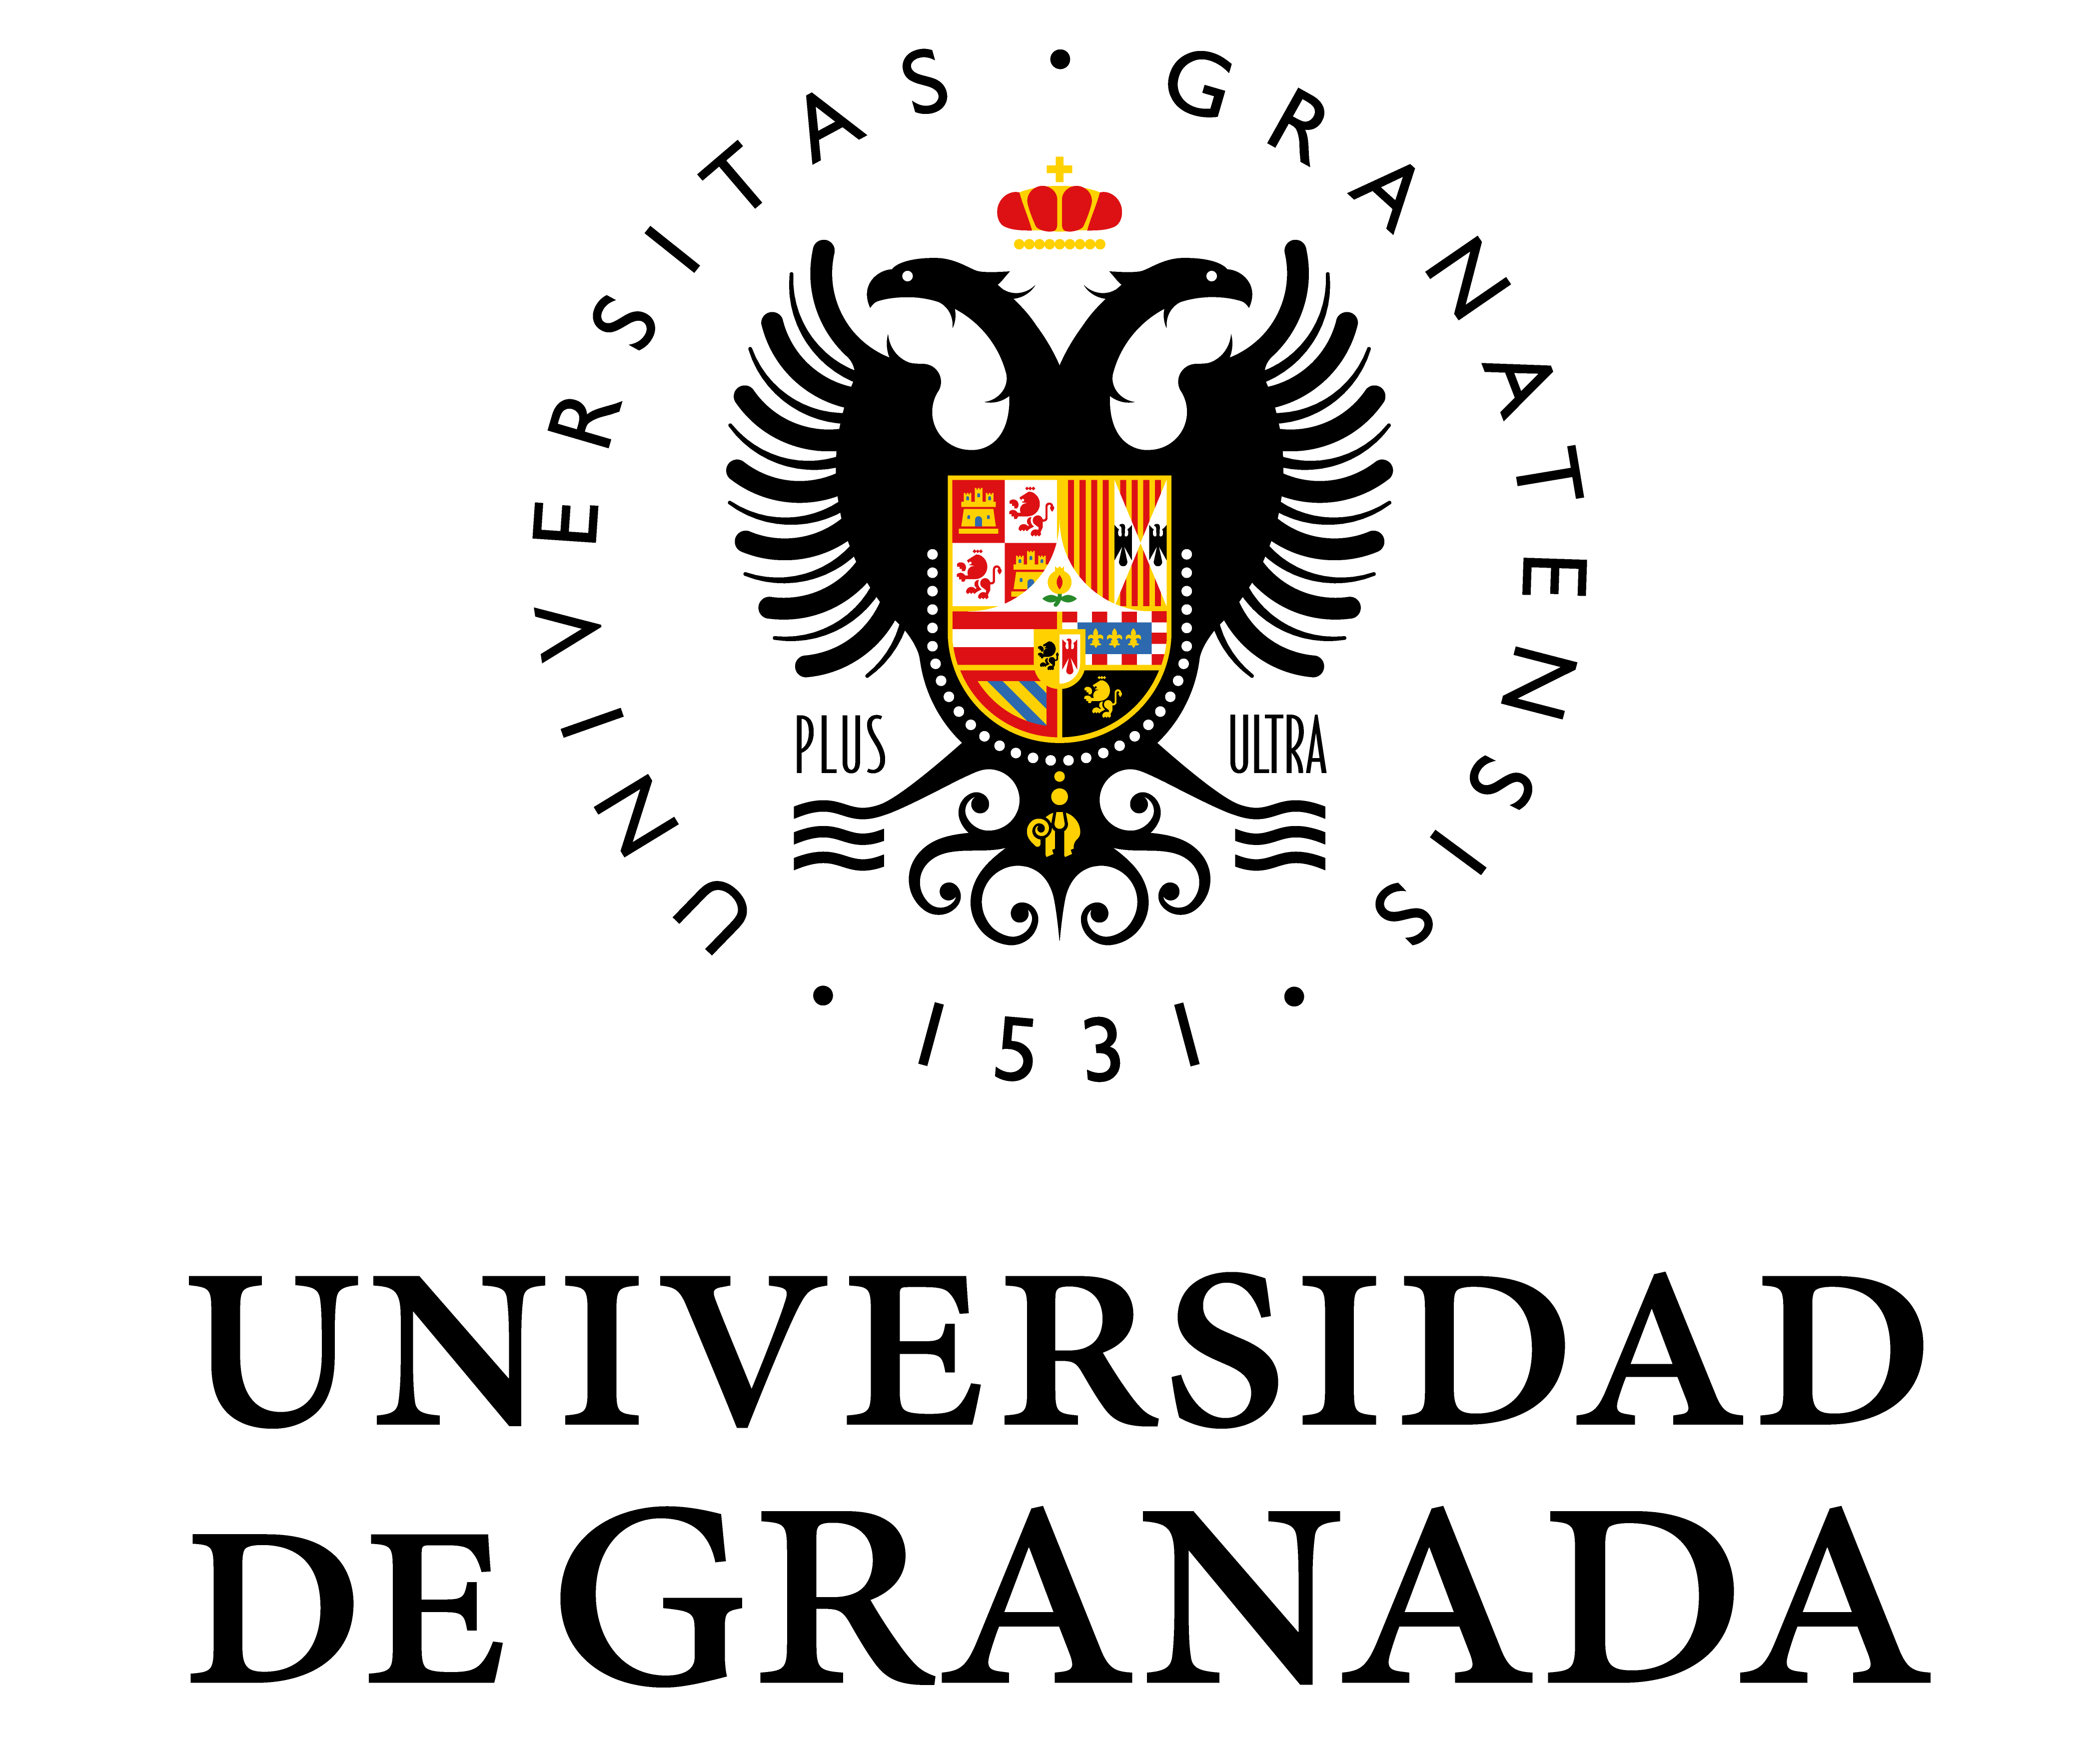
\includegraphics[scale=0.5]{Logo_UGR.png}\par}
	\vspace{1cm}
	{\bfseries\Large Science Faculty \par}
	\vspace{0.5cm}
	{\bfseries\itshape\large Multivariate Statics \par}
	\vspace{2.5cm}
	{\scshape\Huge Influence of diverse indicators in the diagnosis of breast cancer\par}
	\vspace{3cm}
	{\itshape\Large Bachelor's degree in Computer Science and Mathematics}
	\vfill
	{\Large Authors: \par}
	{\Large Julián Garrido Arana \par}
	{\Large Javier Gómez López \par}
	{\Large Juan Valentín Guerrero Cano \par}
	
	\vfill
	{\Large Course 2023-2024 \par}
\end{titlepage}

\thispagestyle{empty}
\null
\vfill

%%Información sobre la licencia
\parbox[t]{\textwidth}{
  
\includegraphics[scale=0.05]{by-nc-sa.png}\\[4pt]
  \raggedright % Texto alineado a la izquierda
  \sffamily\large
  {\Large This work is distributed under a CC BY-NC-SA 4.0 license.}\\[4pt]
  You are free to distribute and adapt the material as long as you acknowledge\\
  the original authors of the document, do not use it for commercial purposes,\\
  and distribute it under the same license.\\[4pt]
  \texttt{creativecommons.org/licenses/by-nc-sa/4.0/}
}

\newpage

\tableofcontents

\newpage

\section{Abstract}
This study responds to the urgent need for a comprehensive understanding of factors influencing breast cancer diagnosis, a disease with substantial global health implications. Employing advanced statiscal techniques such as discriminant analysis, factorial analysis for dimensional reduction, and principal component analysis, the research aims to identify key indicators for more accurate breast cancer classification. \\

By improving diagnostic precision, the study contributes to early and personalized interventions. Additionaly, it seeks to unravel complex interrelationships among various indicators, offering potential insights for advancements in breast cancer research. In essence, this work addresses the practival imperative to enhance breast cancer diagnostics and contributes to ongoing efforts in understanding the intricate aspects of this disease, ultimately advancing medical knowledge and breast cancer treatment.

\newpage

\section{Introduction}
In the intricate realm of breast cancer, the quest for precise diagnosis demands a sophisticated analytical approach that transcends conventional methods. This study embarks on a meticulous exploration, leveraging advanced statistical techniques—discriminant analysis, dimensionality reduction through factorial analysis, and principal component analysis. Our focus centers on unraveling the intricate tapestry of morphological indicators within breast cancer datasets, specifically those linked to diverse sample forms across various cancers.

The amalgamation of genetic, clinical, and morphological indicators necessitates a nuanced statistical lens. Through discriminant analysis, we aim to unveil distinctive morphological patterns characterizing benign and malignant tumors, pushing the boundaries of traditional diagnostic methods. Simultaneously, the application of factorial and principal component analyses enables us to distill essential information from the complex dataset, shedding light on the mathematical factors that truly drive breast cancer classification.

This statistical exploration transcends immediate diagnostic applications. By identifying morphological indicators tied to diverse cancer samples, we not only enhance diagnostic precision but also contribute to a deeper mathematical understanding of the underlying relationships governing the manifestation of different forms of breast cancer. This statistical lens empowers us to navigate the complexities of the disease, unveiling hidden mathematical patterns and connections that may inform novel avenues of research.

In this journey, our objective is twofold: to refine breast cancer diagnosis by identifying morphological indicators associated with various cancer forms through advanced statistical analyses and to contribute to a broader mathematical understanding of the intricate relationships within the disease. As we dissect the statistical nuances associated with morphological variations, we envision a future where mathematical tools are not only more precise but also inherently adaptable to the diverse manifestations of breast cancer. Through this statistical lens, our exploration aspires to redefine the mathematical paradigm of breast cancer diagnosis, providing a foundation for more effective interventions and advancing the collective mathematical understanding of this complex and multifaceted disease.

This study aims to refine breast cancer diagnosis by identifying morphological indicators associated with various cancer forms through advanced statistical analyses, simultaneously contributing to a broader mathematical understanding of the intricate relationships within the disease.

\newpage

\section{Materials and Methods}
\subsection{Materials}

For this study, we have used a public Data Base published by the University of California, at its Machine Learning Repository. This database contains information about 30 `different' features measured through 569 instances of breast cancers. In fact, we do not have 30 features, we have 10, but because most of them refers to spatial measures, we have 3 for each one of this type (\(x,y,z\)). The ten real-valued feautres are computed for each cell nuclues:

\begin{itemize}
	\item Radius (mean of distances from center to points on the perimeter).
	\item Texture (standard deviation of gray-scale values).
	\item Perimeter.
	\item Area.
	\item Smoothness (local variation in radius lengths).
	\item Compactness (\(perimeter^2\) / \(area - 1.0\)).
	\item Concavity (severity of concave portions of the contour).
	\item Symmetry.
	\item Fractal dimension ("coastline approximation" - 1).
\end{itemize}

Due to the size of the features, we recommend to consult the \texttt{R} report of this work to see a summary of the principal position, dispersion and form measures of the features of the database. The table is at section 2.3, where we can find all this interest data.

\subsection{Statiscal methods}


\subsubsection{Univariate exploratory analysis}
First of all we have conducted an \textbf{univariate exploratory analysis}. Regarding the types of values we have on the dataset, we are not interested on perform any type of data-grouping.

We computed the porcentge of missing values, and we saw that there are not missing values. \\

Secondly, we went trough a classical numeric descriptive analysis where the basic numerical descriptive statistics such as principal position, dispersion and form measures were given. We also computed their histograms, boxplots and density graphs. \\

Thirdly, we tried to identify extreme values or outliers. Firstly, we standarized the data to avoid the different scales of our feautres. The decision took for the outliers were to substitute them with the median, due it works better than substituting with the mean. \\

Lastly, to avoid the assumption of normality, we checked the distribution of each feature of the dataset. We did it in a graphical way and using the Shapiro-Wilk test.

\subsubsection{Multivariate Exploratory Analysis}
First of all, we checked some conditions that are necessary to apply the different multivariate analysis techniques:

\begin{itemize}
	\item It is necessary to check if the variables are or no independent. At popultation level, we checked \textbf{correlation} using \textit{Bartlett's Test}.
	\item We also checked the multivariant normality, using the \textit{Henze-Zirkler} test and \textit{Royston} test. It is important to remark that these tests could be perturbated because the presence of outliers, so we had to eliminate them.
\end{itemize}

Once checked all this conditions, we had applied different techniques of Multivariant Analysis. We conducted a \textbf{Principal Component Analysis (PCA)} to reduce the dimension of the problem using observable  variables. After it, we made a \textbf{Factorial Analysis} to identify potential \textit{latent variables} (no observable) that have a high correlation with a group of observable variables and no correlation with the others. Lastly, we performed a \textbf{Discriminant Analysis} (\textbf{Linear} and \textbf{Quadratic}) to establish a classification method of new observations of a cualitative variable according to its characteristics (predictors).

\newpage

\section{Materials and Methods}

\subsection{Database's description}

This dataset contains information about breast cancer cell nuclei, with features computed from digitized images of fine needle aspirates (FNA) of breast masses. The dataset is collected from 569 patients based on 10 different indicators of breast cancer. It has three different measures for each indicator, each one corresponding to a spacial dimensions (XYZ axis). \\

Therefore, the whole dataset  is made up of 569 samples and 30 features, plus two additional features that are the ID (it is not interesting in our case) and the Diagnosis (target of the study).\\


The ten real-valued features for each cell nucleusa are the followings: \\

\begin{itemize}
	\item Radius (mean of distances from center to points on the perimeter)
	\item Texture (standard deviation of gray-scale values)
	\item Perimeter
	\item Area
	\item Smoothness (local variation in radius lengths)
	\item Compactness ($\frac{\text{perimeter}^2}{\text{area} - 1.0}$)
	\item Concavity (severity of concave portions of the contour)
	\item Concave points (number of concave portions of the contour)
	\item Symmetry
	\item Fractal dimension ("coastline approximation" - 1)
\end{itemize}


These features describe characteristics of cell nuclei. The dataset was obtained from images available at \url{http://www.cs.wisc.edu/~street/images/}. \\

On the following table there are some important statistics measures for our dataset that could be interesting to know. 

\begin{figure}[h]
	\centering
	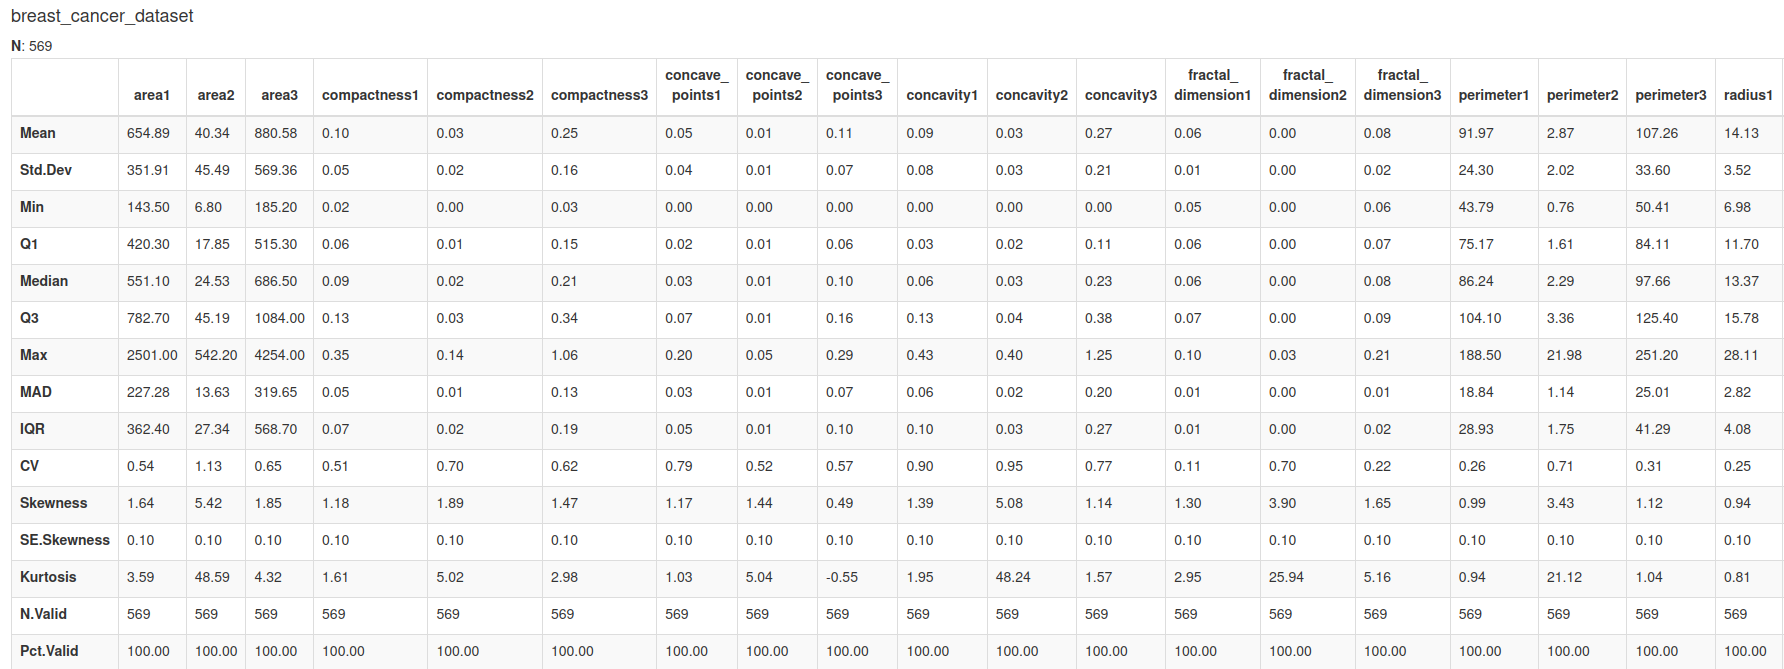
\includegraphics[width=1\textwidth]{statistics_measures}
	\caption{Principal measures for some features.}
	\label{fig:etiqueta}
\end{figure}

NOTE: As the number of features is too high to show all the measures, we have just attached the table with some of them.

\subsection{Statistical methods}

Our proyect has been divided in different sections, where we apply different statistical methods, which will help us to interpretate the results and achieve a better performance. \\


At the beginning, along the second section  we have applied a \textbf{univariate} exploratory analysis, to be aware of what types of data we are working on. More precisely:

\begin{itemize}
	\item \textbf{Missing values:} we have studied the presence of missing values on all the features of our dataset, although we have not found anyone.  If there were any missing value we would analyze the random patterns on them. For that as we have continuous variables we would have applied a Student test, and then replacing them by the mean or median.
	
	\item \textbf{Outliers:}  As some methods we apply along our proyect are sensitive to the presence of outliers we have identified the outliers in each feature. As we have found too many outliers, we have decided to replace them by the mean, as this option was the one which gave us better results. 
	
	
	\item \textbf{Classical numeric descriptive analysis:} For each feature we have computed a "summary" of some interesting statistics measures such as Minimun value, First Quantile, Median, Mean, Third Quantile and Maximum value. Furthermore, we have plot the histograms of each feature, their density and boxplot for a better understanding of the dataset.
	
	\item \textbf{Univariate normality:} as many techniques can not avoid the assumption of normality, we have checked the distribution of each feature of our dataset using two different methods. One which is graphical, using the function qqplot, and the second which apply the Shapiro-Wilk test.\\
	
\end{itemize}

Secondly we have performed a \textbf{multivariate} exploratory analysis using different techniques such as: 

\begin{itemize}
	\item \textbf{Correlation:} we have studied the correlation between the features at two different levels; samplet level, with the corresponding correlation matrix, and at population level, with the Berlett's test. 
	
	\item \textbf{Multivariate normality:} in order to check if the distribution of our data follows a multivariate normal distribution we have performed some test to check  this assumption. We have applied the Royston's test and the Henze-Zirkler's test. Previuosly, we have dealt with the presence of the outliers as we know that these tests are sensitive to the presence of the outliers.
	
\end{itemize}

After checking all these assumptions, we have applied some other methods that will give us the principal results of the proyect, such as Principal Componente Analysis, Factorial Analysis, Linear Discriminant Analysis and Quadratic Discriminant Analysis for building a classification model. Additionally, the Cluster Analysis has been done to complete our research. We will explain all these techniques more precisely along the following sections.

\newpage

\section{Results}

In this section, we will examine the results of the previously mentioned methods from an objective standpoint. \\

Firstly, it is remarkable that we have not dealt with missing values as we have not them  in our dataset. Meanwhile, for the outliers, as explained before, we have replace them by the mean value of each feature. We have considered as outliers the values that are not inside the interquartile range (IQR). \\


The \textbf{univariate normality analysis} have shown that almost every feature of our dataset does not follow a normal distribution. Apart of graphics plot (qq-plots) the Shapiro-Wilk test gave us for each feature a p-value smaller than 0.05 (except for the feature "smoothness1"). \\

\begin{figure}[h]
	\centering
	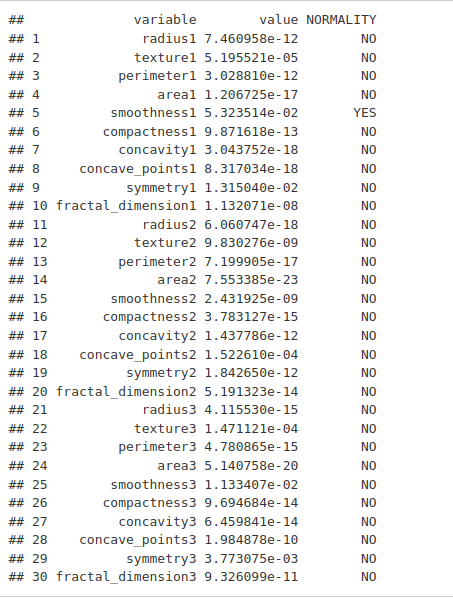
\includegraphics[width=0.4\textwidth]{shapiro_wilktest.png}
	\caption{Results of Shapiro-Wilk test.}
	\label{fig:etiqueta2}
\end{figure}

Regarding the independence of the variables, the \textbf{correlation} method at sample level has given us a correlation matrix with almost non-zero coefficients. Even, we can find high correlation coefficients between some features. Applying \textbf{the Bartlett's sphericity test} for studying the correlation at population level, we have reach that the null hypothesis is rejected (we obtained a p-value of 0). Therefore, we can conclude after these results that the features of our dataset are correlated, and therefore not independent.  \\

 
Therefore, as the features are mainly correlated, it is logical to apply a dimensionaly reduction through PCA or FA:
%TODO (KERCHAK) EXPLICAR LOS RESULTADOS OBJETIVAMENTE 
\begin{itemize}
	\item \textbf{Principal Component Analysis:}
	
	\item \textbf{Factorial Analysis:}\\
	
\end{itemize} 

Finally, we have proceeded with the \textbf{Discriminant Analysis}. For ensuring the 
veracity of the results of the different discriminant analysis methods that we have applied, we have studied again (but this time with the target variable) the univariate  normality of the data. The results have been the same, and for the multivariate normality too. Therefore, despite the lack of normality in our whole dataset, we built the two models (linear and quadratic) for the Discriminant Analysis. It is remarkable that in the following section we will address these issues and how can we interpretate these results.  

\begin{itemize}
	\item \textbf{Linear Discriminant Analysis:}
	
	\item \textbf{Quadratic Discriminant Analysis:}\\
	
\end{itemize} 

The following attached images presents a comparison between the results obtained from these Discriminant Analysis methods.


%TODO(NOTE)


\section{Discussion}

Along this section we will interpretate the different results obtained, and which decisions we have made in each step of the process. \\

Once the data have been preprocessed, we have studied the correlation between variables. As the results were clearly enough to say that our features were not independent, we have made a PCA and FA in order to reduce the dimension of our dataset. \\

%TODO (KERCHAK) INTERPRETAR UN POCO LOS RESULTADOS OBTENIDOS EN PCA Y FA



Before continue with the next steps, we needed to decide if we should finally reduce the dimension of our dataset or not. We decided not to reduce the dimension of our dataset, basing our decision in two key factos: the dimension of our dataset (30 features) is not huge enough to make the computational cost too high, so regarding this factor it is not necessary to reduce dimension. The other factor was the nature of our dataset; as we were stuying medical features, we were not interesting in taking less features by making combination of them. This would lead in "not interpetable" features and in this study we are not interesting in losing the capacity of interpretate each feature. Therefore, despite we have made the study of PCA and FA, the following results are obtained regarding that we have not made dimensionaly reduction. \\


%TODO INTERPRETACION CON YANDEL SOBRE SU DISCRIMINANT ANALYSIS%
Finally, 


\section{Conclusion}

After, this riguruous analysis of the data  we can conclude some imporant facts. Firstly, the dataset was hard to work with, as the most part of the results obtained from the different test were the opposite of what we could expect. Secondly, we have learnt that despite applying dimensionality reduction could be interesting in some cases, in our case it was not too much interesting, as we wanted to be able to interprate the features at the final, as the variables of the dataset were precise measures of the diseases. \\

Another fact we have noticed along the proyect has been that not every dataset will produce the same results, and not what we "want" to get. In real life, the studies will be done in datasets that probably will not follow the "rules" we expect, and therefore, we have to be careful with the results we obtained for the models for example, as the might be not too much reliable.\\

To sum up, this proyect has allowed us to know more about the multivariate analysis of real problems, and to learn how to adapt our interpretation to unexpected results. It is remarkable, that the way this proyect it is focused will help us in the future too for machine learning proyect, to make the right statistical analysis for the data, and to make right interpretations of the prediction model. \\


 





\end{document}
